
\section*{Resources \& Networking}
\DefineNamedColor{named}{eclipsered}{rgb}{0.386,0.366,0.682}
\definecolor{tablecolor}{named}{eclipsered}



\begin{eptable}{ l | X }
   \epheader{2}{Resource Trait}
   Level 1 & Acquire Minor gear in appropriate time frame.\\
   Level 2 & Acquire Moderate gear in appropriate time frame.\\
   Level 3 & Acquire Major gear in appropriate time frame.\\
   Level 4 & Acquire even rare and restricted items (pending GM).\\
\end{eptable}

\begin{itemize}
    \itembox In general cases it is just a matter of
    waiting. In special cases a \skill{Persuation} test may be needed.
    \itembox At Level 3 and Level 4 can be used with Flex to immediately
            acquire Moderate items and introduce them to the scene.
    \itembox High traits can also be used as bribing modifier in
        certain situations. Apply \modifier{+10} per level of trait.
    \itembox Resource trait also reflects player's general life style.
    \itembox Changes in trait due to gameplay should be counter-balanced by Rez cost or award.
\end{itemize}

\begin{eptable}{ l | X }
   \epheader{2}{Lifestyle}
   Level 1 & Own cubicle in a beehive hab or a small apartment.\\
   Level 2 & Private residence or a condo. Small vehicle.\\
   Level 3 & Large residential complex or multiple homes, one or more vehicles.\\
   Level 4 & Rich, might own a small private hab and even shuttle.\\
\end{eptable}

\bigskip

\begin{figure}[htb!]%
   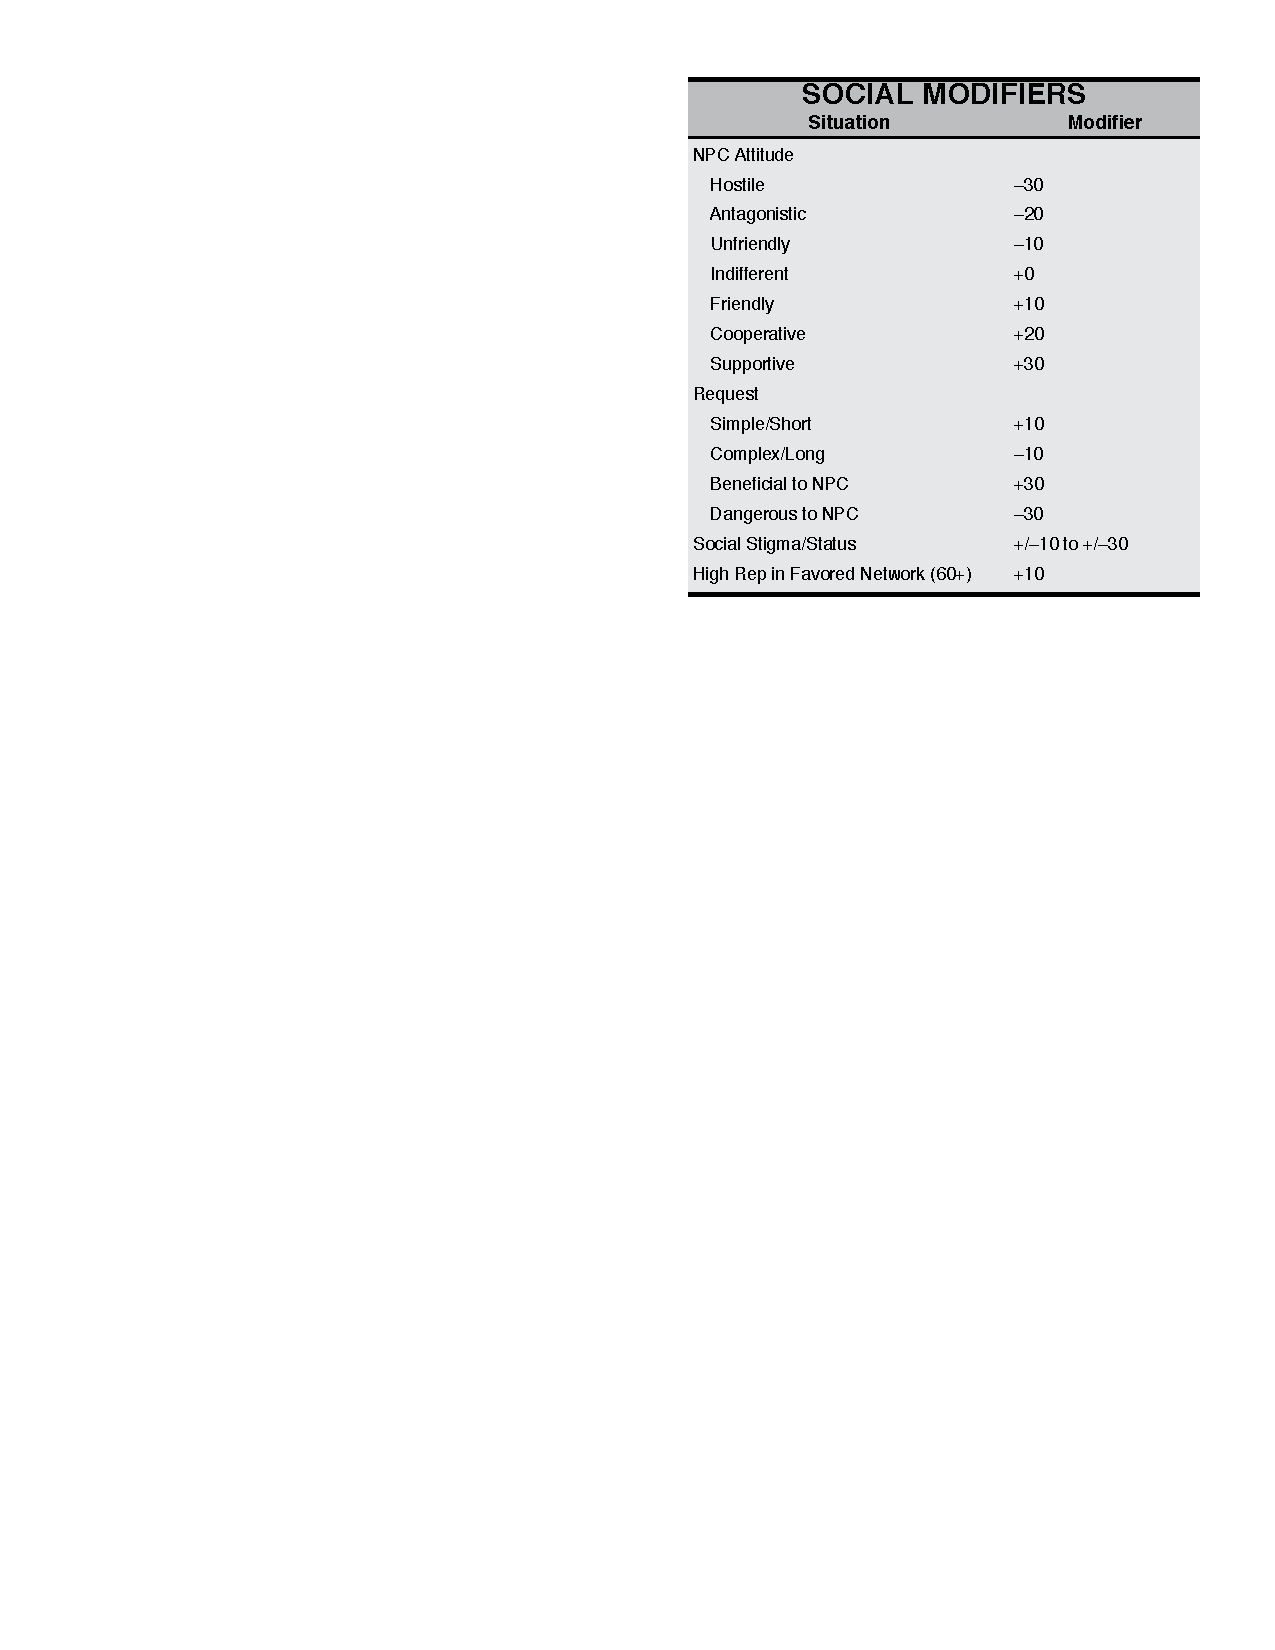
\includegraphics[scale=0.95]{gfx/combat-social-modifiers}%
\end{figure}%



\begin{eptable}{ l | X }
   \epheader{2}{Gear Complexity}
   Minor & Common and easily accessible.\\
   Moderate & Less common, might take time to track down.\\
   Major & Expensive and hard to find.\\
   Rare & Unique, highly unusual or highly valuable.\\
   Restricted & Illegal. Needs special permit or creativity to get. \\
\end{eptable}


\bigskip


\begin{eptable}{ l | X }
   \epheader{2}{Ways to Acquire Gear}
   Rep & Succeed on Rep test and use appropriate favor.\\
   Resource Trait & Use your resources to buy it.\\
   Fabricator & Needs blueprints and access to fabber.\\
\end{eptable}

\begin{itemize}
    \itembox Using Rep to acquire an item uses a favor of the
    equivalent level (\eg, Minor item for Minor favor).
\end{itemize}

\bigskip


\begin{eptable}{ l | X }
   \epheader{2}{Acquisition Time Frame}
   Digital Only & \num{1} minute.\\
   Minor & \num{2} hours.\\
   Moderate & \num{8} hours.\\
   Major & \num{24} hours.\\
   Rare, Restricted & GM choice.\\
\end{eptable}

\begin{itemize}
    \itembox When acquiring gear, chose between actual item or single-use blueprint.
    \itembox Multi-use blueprints are available, but increase complexity by one step.
    \itembox Regular blueprints are assumed to come with one physical copy.
    \itembox Acquiring multiple items combines time frame.
    \itembox When not under time pressure, players should be able
        to acquire regular gear they would have regular access to
        without test.
\end{itemize}

\bigskip

\begin{eptable}{ l | X }
   \epheader{2}{Rep Modifiers}
   Trivial Favor & Reputation test \modifier{+30}, or no test when Rep 60+.\\
   Minor & Reputation test \modifier{+10} \\
   Moderate & Reputation test \modifier{+0} \\
   Major & Reputation test \modifier{-30} \\
\end{eptable}

\begin{itemize}
    \itembox Reputation is rolled like a skill would be rolled with the value in the network.
\end{itemize}

\begin{eptable}{ l | l | X }
   \epheader{3}{Rep Refresh \& Burning }
   Trivial Favor & - & Any time, no limits. \\
   Minor Favor & 5 rep to burn & \num{3} times per week. \\
   Moderate Favor & 10 rep to burn & Once per week. \\
   Major Favor & 20 rep  to burn & Once per campaign. \\
\end{eptable}

\begin{itemize}
    \itembox Favor is not lost on failed test unless critical failure is rolled.
\end{itemize}
